\documentclass[11pt]{article}
\usepackage{amssymb}
\usepackage{amsthm}
\usepackage{enumitem}
\usepackage{amsmath, physics}
\usepackage{bm}
\usepackage{adjustbox}
\usepackage{mathrsfs}
\usepackage{graphicx}
\usepackage{siunitx}
\usepackage[mathscr]{euscript}

\title{\textbf{Solved selected problems of Classical Electrodynamics - Hans Ohanian}}
\author{Franco Zacco}
\date{}

\addtolength{\topmargin}{-3cm}
\addtolength{\textheight}{3cm}

\newcommand{\N}{\mathbb{N}}
\newcommand{\Z}{\mathbb{Z}}
\newcommand{\Q}{\mathbb{Q}}
\newcommand{\R}{\mathbb{R}}
\newcommand{\diam}{\text{diam}}
\newcommand{\cl}{\text{cl}}
\newcommand{\bdry}{\text{bdry}}
\newcommand{\inter}{\text{int}}
\newcommand{\hatx}{\bm{\hat{x}}}
\newcommand{\haty}{\bm{\hat{y}}}
\newcommand{\hatz}{\bm{\hat{z}}}
\newcommand{\hatr}{\bm{\hat{r}}}
\newcommand{\hatn}{\bm{\hat{n}}}
\newcommand{\hatrho}{\bm{\hat{\rho}}}
\newcommand{\hatphi}{\bm{\hat{\phi}}}
\newcommand{\hattheta}{\bm{\hat{\theta}}}


\theoremstyle{definition}
\newtheorem*{solution*}{Solution}
\renewcommand*{\proofname}{\bf{Solution}}

\begin{document}
\maketitle
\thispagestyle{empty}

\section*{Chapter 1 - Vector Calculus}

\subsection*{Exercises}

\begin{proof}{\textbf{Exercise 1.}}
    Verification of
    $\hatx \cdot \hatx = \haty \cdot \haty = \hatz \cdot \hatz = 1$
    \begin{align*}
        \hatx \cdot \hatx = 1 \cdot 1 + 0 \cdot 0 + 0 \cdot 0 = 1\\
        \haty \cdot \haty = 0 \cdot 0 + 1 \cdot 1 + 0 \cdot 0 = 1\\
        \hatz \cdot \hatz = 0 \cdot 0 + 0 \cdot 0 + 1 \cdot 1 = 1
    \end{align*}
    Verification of
    $\hatx \cdot \haty = \hatx \cdot \hatz = \haty \cdot \hatz = 0$
    \begin{align*}
        \hatx \cdot \haty = 1 \cdot 0 + 0 \cdot 1 + 0 \cdot 0 = 0\\
        \hatx \cdot \hatz = 1 \cdot 0 + 0 \cdot 0 + 0 \cdot 1 = 0\\
        \haty \cdot \hatz = 0 \cdot 0 + 1 \cdot 0 + 0 \cdot 1 = 0
    \end{align*}
\end{proof}
\cleardoublepage
\begin{proof}{\textbf{Exercise 2.}}
    We want to verify that the components of Eq. (15) agree
    with those of Eq. (13).
    Let us write the implicit summation for the 1st component as follows
    \begin{align*}
        \varepsilon^{1lm}x^lx'^m &=
        \varepsilon^{111}x^1x'^1 + \varepsilon^{112}x^1x'^2
        + \varepsilon^{113}x^1x'^3 + \\
        &\quad\varepsilon^{121}x^2x'^1 + \varepsilon^{122}x^2x'^2
        + \varepsilon^{123}x^2x'^3 +\\
        &\quad\varepsilon^{131}x^3x'^1 + \varepsilon^{132}x^3x'^2
        + \varepsilon^{133}x^3x'^3\\
        &= \varepsilon^{123}x^2x'^3 + \varepsilon^{132}x^3x'^2\\
        &= x^2x'^3 - x^3x'^2
    \end{align*}
    We see that it agrees with the first component of Eq. (13).
    In the same way, for the 2nd and 3rd components, we have that
    \begin{align*}
        \varepsilon^{2lm}x^lx'^m &=
        \varepsilon^{211}x^1x'^1 + \varepsilon^{212}x^1x'^2
        + \varepsilon^{213}x^1x'^3 + \\
        &\quad\varepsilon^{221}x^2x'^1 + \varepsilon^{222}x^2x'^2
        + \varepsilon^{223}x^2x'^3 +\\
        &\quad\varepsilon^{231}x^3x'^1 + \varepsilon^{232}x^3x'^2
        + \varepsilon^{233}x^3x'^3\\
        &= \varepsilon^{213}x^1x'^3 + \varepsilon^{231}x^3x'^1\\
        &= x^3x'^1 - x^1x'^3\\
        \varepsilon^{3lm}x^lx'^m &=
        \varepsilon^{311}x^1x'^1 + \varepsilon^{312}x^1x'^2
        + \varepsilon^{313}x^1x'^3 + \\
        &\quad\varepsilon^{321}x^2x'^1 + \varepsilon^{322}x^2x'^2
        + \varepsilon^{323}x^2x'^3 +\\
        &\quad\varepsilon^{331}x^3x'^1 + \varepsilon^{332}x^3x'^2
        + \varepsilon^{333}x^3x'^3\\
        &= \varepsilon^{312}x^1x'^2 + \varepsilon^{321}x^2x'^1\\
        &= x^1x'^2 - x^2x'^1
    \end{align*}
\end{proof}
\begin{proof}{\textbf{Exercise 3.}}
    We know that the $k$-th component of $\bm{x} \times \bm{x}'$ is given 
    $[\bm{x} \times \bm{x}']^k = \varepsilon^{klm}x^lx'^m$. Also, we know
    that $\varepsilon^{123} = \varepsilon^{231} = \varepsilon^{312} = 1$
    and that $\varepsilon^{213} = \varepsilon^{132} = \varepsilon^{321} = -1$
    this implies that if we swap any two superscripts we invert
    the sign, so we have that $\varepsilon^{klm} = -\varepsilon^{kml}$.
    From this, we have that
    \begin{align*}
        [\bm{x} \times \bm{x}']^k &= \varepsilon^{klm}x^l x'^m\\
            &= -\varepsilon^{kml}x^l x'^m\\
            &= -\varepsilon^{kml}x'^m x^l\\
            &= -[\bm{x}' \times \bm{x}]^k
    \end{align*}
\end{proof}
\cleardoublepage
\begin{proof}{\textbf{Exercise 4.}}
    Let us plot the position vector $r$ as follows
    \begin{center}
        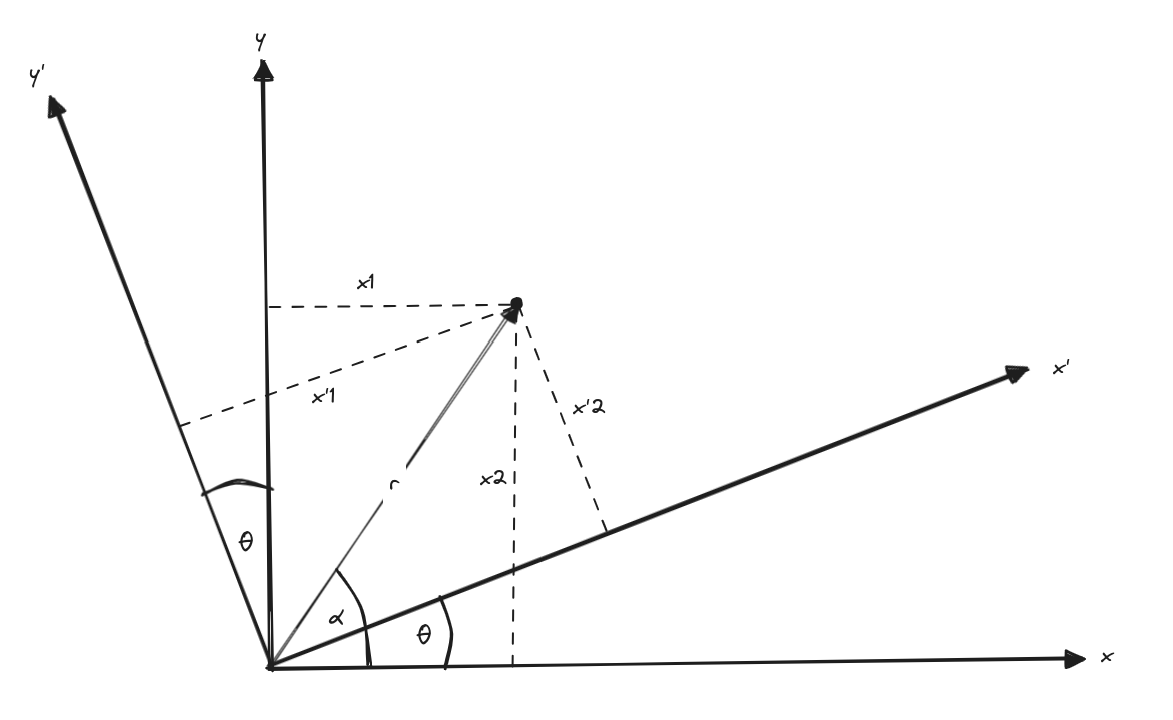
\includegraphics[scale=0.3]{ch1-4.png}
    \end{center}
    Then we see that
    \begin{align*}
        x^1 &= r\cos\alpha\\
        x^2 &= r\sin\alpha\\
        x^3 &= 0
    \end{align*}
    Also, we have that
    \begin{align*}
        x'^1 &= r\cos(\alpha - \theta)\\
        x'^2 &= r\sin(\alpha - \theta)\\
        x'^3 &= 0
    \end{align*}
    Hence by the trigonometric identities, we get that
    \begin{align*}
        x'^1 = r\cos\alpha\cos\theta + r\sin\alpha\sin\theta\\
        x'^2 = r\sin\alpha\cos\theta - r\cos\alpha\sin\theta
    \end{align*}
    Therefore
    \begin{align*}
        x'^1 &= x^1\cos\theta + x^2\sin\theta\\
        x'^2 &= x^2\cos\theta - x^1\sin\theta\\
        x'^3 &= x^3
    \end{align*}
\end{proof}
\cleardoublepage
\begin{proof}{\textbf{Exercise 5.}}
    Let
    \begin{align*}
        x'^k = a^{kn} x^n
    \end{align*}
    Where
    \begin{alignat*}{3}
        a^{11} &= \cos\theta &\quad a^{12} &= \sin\theta &\quad a^{13} &= 0\\
        a^{21} &= -\sin\theta &\quad a^{22} &= \cos\theta &\quad a^{23} &= 0\\
        a^{31} &= 0 &\quad a^{32} &= 0 &\quad a^{33} &= 1\\
    \end{alignat*}
    Hence we have that
    \begin{align*}
        x'^1 &= a^{11}x^1 + a^{12}x^2 + a^{13}x^3\\
            &= x^1 \cos\theta + x^2\sin\theta 
    \end{align*}
    And in the same way
    \begin{align*}
        x'^2 &= a^{21}x^1 + a^{22}x^2 + a^{23}x^3\\
            &= -x^1 \sin\theta + x^2\cos\theta\\
        x'^3 &= a^{31}x^1 + a^{32}x^2 + a^{33}x^3\\
            &= x^3            
    \end{align*}
\end{proof}
\cleardoublepage
\begin{proof}{\textbf{Exercise 6.}}
    Let
    \begin{align*}
        a^{kn} = 
        \begin{pmatrix}
            \cos\theta & \sin\theta & 0\\
            -\sin\theta & \cos\theta & 0\\
            0 & 0 & 1
        \end{pmatrix}
    \end{align*}
    and
    \begin{align*}
        b^{mk} = 
        \begin{pmatrix}
            \cos\phi & \sin\phi & 0\\
            -\sin\phi & \cos\phi & 0\\
            0 & 0 & 1
        \end{pmatrix}
    \end{align*}
    Then $c^{mn}$ is given by
    \begin{align*}
        c^{mn} &= 
        \begin{pmatrix}
            \cos\phi & \sin\phi & 0\\
            -\sin\phi & \cos\phi & 0\\
            0 & 0 & 1
        \end{pmatrix}
        \cdot
        \begin{pmatrix}
            \cos\theta & \sin\theta & 0\\
            -\sin\theta & \cos\theta & 0\\
            0 & 0 & 1
        \end{pmatrix}\\
        &= 
        \begin{pmatrix}
            \cos\phi\cos\theta - \sin\phi\sin\theta
            & \cos\phi\sin\theta + \sin\phi\cos\theta
            & 0\\
            -\sin\phi\cos\theta - \cos\phi\sin\theta
            & -\sin\phi\sin\theta + \cos\phi\cos\theta
            & 0\\
            0 & 0 & 1
        \end{pmatrix}\\
        &=
        \begin{pmatrix}
            \cos(\phi +\theta) & \sin(\phi + \theta) & 0\\
            -\sin(\phi + \theta) & \cos(\phi + \theta) & 0\\
            0 & 0 & 1
        \end{pmatrix}
    \end{align*}
    Where we used that
    $\sin(\phi \pm \theta) = \sin\phi\cos\theta \pm \cos\phi\sin\theta$
    and that
    $\cos(\phi \pm \theta) = \cos\phi\cos\theta \mp \sin\phi\sin\theta$.
    Finally, we expect to have the sum of the angles $\phi$ and $\theta$ since
    the entire transformation implies a final rotation of an angle $\phi + \theta$.  
\end{proof}
\begin{proof}{\textbf{Exercise 7.}}
    Let $x^l \neq 0$ and let $x^m = x^l$ then if $a^{km}a^{kl} \neq \delta^{ml}$
    we have that
    \begin{align*}
        x^lx^m(a^{km}a^{kl} - \delta^{ml}) \neq 0
    \end{align*}
\end{proof}
\begin{proof}{\textbf{Exercise 8.}}
    Given that $A^k$ and $B^k$ are vectors then they transform under rotations
    as follows
    \begin{align*}
        A'^k = a^{kn} A^n \quad\text{and}\quad B'^k = a^{kn} B^n
    \end{align*}
    Let us define $C^n = \alpha A^n + \beta B^n $
    then by multiplying $C^n$ by $a^{kn}$ we get that
    \begin{align*}
        a^{kn}C^n &= a^{kn}(\alpha A^n + \beta B^n)\\
            &= \alpha a^{kn} A^n + \beta a^{kn}B^n\\
            &= \alpha A'^k + \beta B'^k\\
            &= C'^k
    \end{align*}
    Hence $C^n$ also transforms in the same way under rotations.
    This implies that $C^n = \alpha A^n + \beta B^n$ is also a vector.
\end{proof}
\begin{proof}{\textbf{Exercise 9.}}
    Given that $T^{kl}$ and $Q^{kl}$ are tensors then they transform under
    rotations as follows
    \begin{align*}
        T'^{kl} = a^{kn}a^{lm} T^{nm} \quad\text{and}\quad
        Q'^{kl} = a^{kn}a^{lm} Q^{nm}
    \end{align*}
    Let us define $C^{nm} = \alpha T^{nm} + \beta Q^{nm} $
    then by multiplying $C^{nm}$ by $a^{kn}a^{lm}$ we get that
    \begin{align*}
        a^{kn}a^{lm}C^{nm} &= a^{kn}a^{lm}(\alpha T^{nm} + \beta Q^{nm})\\
            &= \alpha a^{kn}a^{lm} T^{nm} + \beta a^{kn}a^{lm}Q^{nm}\\
            &= \alpha T'^{kl} + \beta Q'^{kl}\\
            &= C'^{kl}
    \end{align*}
    Hence $C^{nm}$ also transforms in the same way under rotations.
    This implies that $C^{nm} = \alpha T^{nm} + \beta Q^{nm}$ is also a tensor.
\end{proof}
\begin{proof}{\textbf{Exercise 10.}}
    Multiplying $\delta^{nm}$ by $a^{kn}a^{lm}$ we have that
    \begin{align*}
        a^{kn}a^{lm}\delta^{nm}
        = a^{km}a^{lm} = a^{km}(a^{T})^{ml} = \delta^{kl}
    \end{align*}
    where we used that $a^{kn}\delta^{nm} = a^{km}$ and that
    $a^{lm} = (a^{T})^{ml}$. Therefore the Kronecker delta is a tensor.
\end{proof}
\begin{proof}{\textbf{Exercise 11.}}
    We know that $(T'^{T})^{kl} = T'^{lk}$ so we have that
    \begin{align*}
        (T'^{T})^{kl} = T'^{lk} = a^{lm}a^{kn} T^{mn} = a^{kn}a^{lm} (T^{T})^{nm}
    \end{align*}
    Where we changed from $a^{lm}a^{kn}$ to $a^{kn}a^{lm}$ since the order of
    multiplication doesn't matter. This implies that the
    transpose of any tensor is a tensor.
\end{proof}
\begin{proof}{\textbf{Exercise 12.}}
    Let $T'^{kl}$ be a tensor and $B'^{l}$ be a vector, we want to show
    $T'^{kl}B^{l}$ is a vector hence by using the transformation laws for
    tensors and vectors we have that
    \begin{align*}
        T'^{kl}B'^{l} &= a^{kn}a^{lm}T^{nm}a^{ld}B^d\\
        &= (a^T)^{ml}a^{ld} a^{kn} T^{nm}B^d\\
        &= a^{kn}T^{nm}\delta^{md}B^d\\
        &= a^{kn}T^{nm}B^m
    \end{align*}
    Therefore $T'^{kl}B'^{l}$ transforms like a vector, and hence it's a vector.
\end{proof}
\begin{proof}{\textbf{Exercise 13.}}
    Let $T'^{kl}$ and $Q'^{ln}$ be tensors, we want to show that
    $T'^{kl}Q'^{ln}$ is a tensor hence by using the transformation laws for
    tensors we have that
    \begin{align*}
        T'^{kl}Q'^{ln} &= a^{kf}a^{lm}T^{fm} a^{ld}a^{nb} Q^{db}\\
        &= a^{kf}a^{nb} T^{fm} (a^{T})^{ml} a^{ld}  Q^{db}\\
        &= a^{kf}a^{nb} T^{fm} \delta^{md}Q^{db}\\
        &= a^{kf}a^{nb} T^{fm} Q^{mb}
    \end{align*}
    Therefore $T'^{kl}Q'^{ln}$ transforms like a tensor, and hence it's a tensor.
\end{proof}

\begin{proof}{\textbf{Exercise 14.}}
    Let $T'^{kl}$ be a tensor, we want to show that
    $T'^{ll}$ is a scalar hence by using the transformation laws for
    tensors we have that
    \begin{align*}
        T'^{ll} &= a^{ln}a^{lm} T^{nm}\\
        &= (a^T)^{nl}a^{lm} T^{nm}\\
        &= \delta^{nm} T^{nm}\\
        &= T^{nn}
    \end{align*}
    Therefore $T'^{ll}$ remains unchanged under rotations so it is a scalar.
\end{proof}
\begin{proof}{\textbf{Exercise 15.}}
    Let $A^k$, $B^l$ and $C^m$ be vectors then they transform as
    $A'^k = a^{kn} A^n$, $B'^l = a^{lr}B^r$ and $C'^m = a^{ms}C^s$ so
    by multiplying them we have that
    \begin{align*}
        A'^k B'^l C'^m = a^{kn}A^n a^{lr}B^r a^{ms}C^s
            = a^{kn} a^{lr} a^{ms} A^n B^r C^s
    \end{align*}
    Then $A^k B^l C^m$ transform like a third rank tensor hence $A^k B^l C^m$
    is a tensor.
\end{proof}
\begin{proof}{\textbf{Exercise 16.}}
    Let $\varepsilon^{klm}$ be the alternating tensor, we want to show it is
    a third-rank tensor i.e. we want to prove that
    \begin{align*}
        \varepsilon'^{klm} = a^{kn}a^{lr}a^{ms} \varepsilon^{nrs}
    \end{align*}
    So let us evaluate explicitly the right side of the above equation for the
    indices $k=1$, $l=2$ and $m = 3$ 
    \begin{align*}
        a^{1n}a^{2r}a^{3s}\varepsilon^{nrs} &= a^{11}a^{22}a^{33}\varepsilon^{123}
        + a^{12}a^{23}a^{31}\varepsilon^{231}
        + a^{13}a^{21}a^{32}\varepsilon^{312}\\
        &\quad+ a^{12}a^{21}a^{33}\varepsilon^{213}
        + a^{11}a^{23}a^{32}\varepsilon^{132}
        + a^{13}a^{22}a^{31}\varepsilon^{321}\\
        &= \cos\theta \cdot \cos\theta \cdot 1 \cdot 1
        + \sin\theta \cdot 0 \cdot 0 \cdot 1
        + 0 \cdot (-\sin\theta) \cdot 0 \cdot 1\\
        &\quad + \sin\theta \cdot (-\sin\theta) \cdot 1 \cdot (-1)
        + \cos\theta \cdot 0 \cdot 0 \cdot (-1)\\
        &\quad + 0 \cdot \cos\theta \cdot 0 \cdot (-1)\\
        &= \cos^2\theta + \sin^2\theta\\
        &= 1
    \end{align*}
    In the same way for $k,l,m=2,3,1$ and $k,l,m = 3,1,2$ 
    \begin{align*}
        a^{2n}a^{3r}a^{1s}\varepsilon^{nrs} &=
        a^{21}a^{32}a^{13}\varepsilon^{123}
        + a^{22}a^{33}a^{11}\varepsilon^{231}
        + a^{23}a^{31}a^{12}\varepsilon^{312}\\
        &\quad+ a^{22}a^{31}a^{13}\varepsilon^{213}
        + a^{21}a^{33}a^{12}\varepsilon^{132}
        + a^{23}a^{32}a^{11}\varepsilon^{321}\\
        &= 0 + \cos^2\theta + 0 + 0 + \sin^2\theta + 0\\
        &= \cos^2\theta + \sin^2\theta\\
        &= 1\\
        a^{3n}a^{1r}a^{2s}\varepsilon^{nrs} &=
        a^{31}a^{12}a^{23}\varepsilon^{123}
        + a^{32}a^{13}a^{21}\varepsilon^{231}
        + a^{33}a^{11}a^{22}\varepsilon^{312}\\
        &\quad+ a^{32}a^{11}a^{23}\varepsilon^{213}
        + a^{31}a^{13}a^{22}\varepsilon^{132}
        + a^{33}a^{12}a^{21}\varepsilon^{321}\\
        &= 0 + 0 + \cos^2\theta + 0 + 0 + \sin^2\theta\\
        &= \cos^2\theta + \sin^2\theta\\
        &= 1
    \end{align*}
    Now we evaluate the equation for $k,l,m = 2,1,3$
    \begin{align*}
        a^{2n}a^{1r}a^{3s}\varepsilon^{nrs} &=
        a^{21}a^{12}a^{33}\varepsilon^{123}
        + a^{22}a^{13}a^{31}\varepsilon^{231}
        + a^{23}a^{11}a^{32}\varepsilon^{312}\\
        &\quad+ a^{22}a^{11}a^{33}\varepsilon^{213}
        + a^{21}a^{13}a^{32}\varepsilon^{132}
        + a^{23}a^{12}a^{31}\varepsilon^{321}\\
        &= -\sin^2\theta + 0 + 0 -\cos^2\theta + 0 + 0\\
        &= -(\cos^2\theta + \sin^2\theta)\\
        &= -1
    \end{align*}
    Thus for $k,l,m = 1,3,2$ and $k,l,m = 3,2,1$
    \begin{align*}
        a^{1n}a^{3r}a^{2s}\varepsilon^{nrs} &=
        a^{11}a^{32}a^{23}\varepsilon^{123}
        + a^{12}a^{33}a^{21}\varepsilon^{231}
        + a^{13}a^{31}a^{22}\varepsilon^{312}\\
        &\quad+ a^{12}a^{31}a^{23}\varepsilon^{213}
        + a^{11}a^{33}a^{22}\varepsilon^{132}
        + a^{13}a^{32}a^{21}\varepsilon^{321}\\
        &= 0 -\sin^2\theta + 0 + 0 -\cos^2\theta + 0\\
        &= -(\cos^2\theta + \sin^2\theta)\\
        &= -1\\
        a^{3n}a^{2r}a^{1s}\varepsilon^{nrs} &=
        a^{31}a^{22}a^{13}\varepsilon^{123}
        + a^{32}a^{23}a^{11}\varepsilon^{231}
        + a^{33}a^{21}a^{12}\varepsilon^{312}\\
        &\quad+ a^{32}a^{21}a^{13}\varepsilon^{213}
        + a^{31}a^{23}a^{12}\varepsilon^{132}
        + a^{33}a^{22}a^{11}\varepsilon^{321}\\
        &= 0 + 0 -\sin^2\theta + 0 + 0 -\cos^2\theta\\
        &= -(\cos^2\theta + \sin^2\theta)\\
        &= -1
    \end{align*}
    Hence the equation matches the non-zero elements of $\varepsilon'^{klm}$.

    Next, we want to show that elements of the form $\varepsilon'^{kkm}$ are
    zero, hence let $k,l =1,1$ then
    \begin{align*}
        a^{1n}a^{1r}a^{ms}\varepsilon^{nrs} &=
        a^{11}a^{12}a^{ms}\varepsilon^{12s}
        + a^{12}a^{11}a^{ms}\varepsilon^{21s}\\
        &= a^{ms}(a^{11}a^{12}\varepsilon^{12s}
        + a^{12}a^{11}\varepsilon^{21s})\\
        &= a^{ms}(a^{11}a^{12} - a^{12}a^{11})\\
        &= 0
    \end{align*}
    In the same way for $k,l =2,2$ we have that
    \begin{align*}
        a^{2n}a^{2r}a^{ms}\varepsilon^{nrs} &=
        a^{21}a^{22}a^{ms}\varepsilon^{12s}
        + a^{22}a^{21}a^{ms}\varepsilon^{21s}\\
        &= a^{ms}(a^{21}a^{22}\varepsilon^{12s}
        + a^{22}a^{21}\varepsilon^{21s})\\
        &= a^{ms}(a^{21}a^{22} - a^{22}a^{21})\\
        &= 0
    \end{align*}
    and for $k,l =3,3$ since no index combination is different from zero we
    have that
    \begin{align*}
        a^{3n}a^{3r}a^{ms}\varepsilon^{nrs} &= 0 
    \end{align*}
    The same can be shown for elements of the form $\varepsilon^{kll}$ and
    $\varepsilon^{mlm}$. Therefore we have shown that
    \begin{align*}
        \varepsilon'^{klm} = a^{kn}a^{lr}a^{ms} \varepsilon^{nrs}
    \end{align*}
\end{proof}
\begin{proof}{\textbf{Exercise 17.}}
    Let $A^l$ and $B^m$ be vectors then they transform as
    $A'^l = a^{lr} A^r$ and $B'^m = a^{ms}B^s$ so we have that
    \begin{align*}
        \varepsilon'^{klm}A'^lB'^m &= a^{kn}a^{lr}a^{ms}\varepsilon^{nrs}a^{lr} A^ra^{ms}B^s\\
            &= a^{kn}a^{lr}(a^T)^{rl}a^{ms}(a^T)^{sm}\varepsilon^{nrs} A^rB^s\\
            &= a^{kn}\delta^{ll} \delta^{mm}\varepsilon^{nrs} A^rB^s\\
            &= a^{kn}\varepsilon^{nrs} A^rB^s
    \end{align*}
    So we see that $\varepsilon^{klm} A^lB^m$ transforms like a vector as we
    wanted.
\end{proof}
\begin{proof}{\textbf{Exercise 18.}}
    Let $\bm B = \nabla\Phi$ where $\Phi$ is a scalar field then
    by switching indices we have that
    \begin{align*}
        \varepsilon^{klm}
        \frac{\partial}{\partial x^l} \frac{\partial \Phi}{\partial x^m}
        &=\varepsilon^{kml}
        \frac{\partial}{\partial x^m} \frac{\partial \Phi}{\partial x^l}\\
        &=\varepsilon^{kml}
        \frac{\partial}{\partial x^l} \frac{\partial \Phi}{\partial x^m}\\
        &= -\varepsilon^{klm}
        \frac{\partial}{\partial x^l} \frac{\partial \Phi}{\partial x^m}
    \end{align*}
    Where we used that
    $\frac{\partial}{\partial x^m} \frac{\partial \Phi}{\partial x^l} 
    = \frac{\partial}{\partial x^l} \frac{\partial \Phi}{\partial x^m}$.
    But this can only be true if 
    \begin{align*}
        \varepsilon^{klm}
        \frac{\partial}{\partial x^l} \frac{\partial \Phi}{\partial x^m}
        &= 0 
    \end{align*}
    Finally, we should be able to obtain the same result making explicit the equation
    $\nabla \times \nabla \Phi$ as follows
    \begin{align*}
        \nabla \times \nabla \Phi &=
        \hat{\bm x} \left(
            \frac{\partial}{\partial x^2}
            \frac{\partial \Phi}{\partial x^3}
            - \frac{\partial}{\partial x^3}
            \frac{\partial \Phi}{\partial x^2}
        \right)
        + \hat{\bm y} \left(
            \frac{\partial}{\partial x^3}
            \frac{\partial \Phi}{\partial x^1}
            - \frac{\partial}{\partial x^1}
            \frac{\partial \Phi}{\partial x^3}
        \right)\\
        &\quad + \hat{\bm z} \left(
            \frac{\partial}{\partial x^1}
            \frac{\partial \Phi}{\partial x^2}
            - \frac{\partial}{\partial x^2}
            \frac{\partial \Phi}{\partial x^1}
        \right)\\
        &= \hat{\bm x} \cdot 0 + \hat{\bm y}\cdot 0 + \hat{\bm{z}}\cdot 0\\
        &= \bm 0
    \end{align*}
\end{proof}
\cleardoublepage
\begin{proof}{\textbf{Exercise 19.}}
    Let $\bm B$ be a vector then the divergence of the curl can be written as
    \begin{align*}
        \frac{\partial}{\partial x^k}\varepsilon^{klm}
        \frac{\partial}{\partial x^l} B^m
        &= \varepsilon^{lkm} \frac{\partial}{\partial x^l}
        \frac{\partial}{\partial x^k} B^m\\
        &= \varepsilon^{lkm} \frac{\partial}{\partial x^k}
        \frac{\partial}{\partial x^l} B^m\\
        &= -\varepsilon^{klm}\frac{\partial}{\partial x^k}
        \frac{\partial}{\partial x^l} B^m\\
        &= -\frac{\partial}{\partial x^k}\varepsilon^{klm}
        \frac{\partial}{\partial x^l} B^m
    \end{align*}
    Where we used that
    $\frac{\partial}{\partial x^k} \frac{\partial }{\partial x^l}B^m 
    = \frac{\partial}{\partial x^l} \frac{\partial }{\partial x^k} B^m$.
    But this can only be true if 
    \begin{align*}
        \frac{\partial}{\partial x^k}\varepsilon^{klm}
        \frac{\partial}{\partial x^l} B^m &= 0 
    \end{align*}
    Finally, we should be able to obtain the same result by making explicit
    the equation $\nabla \cdot (\nabla \times \bm{B}) = 0$ as follows
    \begin{align*}
        \nabla \cdot (\nabla \times \bm{B}) &=
        \frac{\partial}{\partial x} \left(
            \frac{\partial}{\partial y}B_z
            - \frac{\partial}{\partial z}B_y
        \right)
        + \frac{\partial}{\partial y} \left(
            \frac{\partial}{\partial z}B_x
            - \frac{\partial}{\partial x}B_z
        \right)\\
        &\quad + \frac{\partial}{\partial z} \left(
            \frac{\partial}{\partial x}B_y
            - \frac{\partial}{\partial y}B_x
        \right)\\
        &= \frac{\partial}{\partial x}\frac{\partial}{\partial y}B_z
            - \frac{\partial}{\partial x}\frac{\partial}{\partial z}B_y
        + \frac{\partial}{\partial y}\frac{\partial}{\partial z}B_x
            - \frac{\partial}{\partial y}\frac{\partial}{\partial x}B_z
        \\
        &\quad + \frac{\partial}{\partial z}\frac{\partial}{\partial x}B_y
            - \frac{\partial}{\partial z}\frac{\partial}{\partial y}B_x
        \\
        &= 0
    \end{align*}
\end{proof}
\begin{proof}{\textbf{Exercise 20.}}
    \begin{align*}
        \partialderivative{\hatrho}{\phi} &=
        \hatx\partialderivative{\cos\phi}{\phi} + \haty \partialderivative{\sin\phi}{\phi}
        = -\hatx\sin\phi + \haty \cos\phi = \hatphi\\
        \partialderivative{\hatphi}{\phi} &=
        -\hatx\partialderivative{\sin\phi}{\phi}
        + \haty \partialderivative{\cos\phi}{\phi}
        = -\hatx\cos\phi - \haty \sin\phi = -\hatrho
    \end{align*}
\end{proof}
\cleardoublepage
\begin{proof}{\textbf{Exercise 21.}}
    We want to prove that
    $$\nabla = \hatrho \partialderivative{}{\rho}
    + \hatphi \frac{1}{\rho}\partialderivative{}{\phi}
    + \hatz\partialderivative{}{z}$$
    So from this expression, we should be able to get $\nabla$
    in cartesian coordinates.

    First, we need to compute a few partial derivatives that we will need later
    \begin{align*}
        \partialderivative{x}{\rho} &= \cos\phi\quad\quad
        \partialderivative{y}{\rho} = \sin\phi\\
        \partialderivative{x}{\phi} &= -\rho\sin\phi\quad\quad
        \partialderivative{y}{\phi} = \rho\cos\phi
    \end{align*}
    So replacing the partial derivatives we computed and using equation (81),
    we have that
    \begin{align*}
        \nabla &= \hatrho \partialderivative{}{\rho}
        + \hatphi \frac{1}{\rho}\partialderivative{}{\phi}
        + \hatz\partialderivative{}{z}\\
        &= \hatrho \bigg(\partialderivative{}{x}\partialderivative{x}{\rho}
        + \partialderivative{}{y}\partialderivative{y}{\rho}\bigg)
        + \hatphi\frac{1}{\rho}\bigg(
            \partialderivative{}{x}\partialderivative{x}{\phi}
            + \partialderivative{}{y}\partialderivative{y}{\phi}\bigg)
        + \hatz\partialderivative{}{z}\\
        &= \hatrho \bigg(\partialderivative{}{x}\cos\phi
        + \partialderivative{}{y}\sin\phi\bigg)
        + \hatphi\frac{1}{\rho}\bigg(
            -\partialderivative{}{x}\rho\sin\phi
            + \partialderivative{}{y}\rho\cos\phi\bigg)
        + \hatz\partialderivative{}{z}\\
        &= (\hatx\cos\phi + \haty\sin\phi)\bigg(\partialderivative{}{x}\cos\phi
        + \partialderivative{}{y}\sin\phi\bigg) +\\
        &\quad+ (-\hatx\sin\phi + \haty\cos\phi)\frac{1}{\rho}\bigg(
            -\partialderivative{}{x}\rho\sin\phi
            + \partialderivative{}{y}\rho\cos\phi\bigg)
        + \hatz\partialderivative{}{z}\\
        &= \hatx\partialderivative{}{x}\cos^2\phi
        + \hatx\partialderivative{}{y}\sin\phi\cos\phi
        + \haty\partialderivative{}{x}\cos\phi\sin\phi
        + \haty\partialderivative{}{y}\sin^2\phi + \\
        &\quad
        + \hatx\partialderivative{}{x}\sin^2\phi
        - \hatx\partialderivative{}{y}\sin\phi\cos\phi
        - \haty\partialderivative{}{x}\cos\phi\sin\phi
        + \haty\partialderivative{}{y}\cos^2\phi
        + \hatz\partialderivative{}{z}\\
        &= \hatx\frac{\partial}{\partial x}(\cos^2\phi + \sin^2\phi)
        + \haty\frac{\partial}{\partial y}(\cos^2\phi + \sin^2\phi)
        + \hatz\partialderivative{}{z}\\
        &= \hatx\frac{\partial}{\partial x} + \haty\frac{\partial}{\partial y}
        + \hatz\partialderivative{}{z}
    \end{align*}
\end{proof}
\cleardoublepage
\begin{proof}{\textbf{Exercise 22.}}
    We want to compute the following
    \begin{align*}
        \divergence{\bm{A}} =
        \bigg(
            \hatrho \partialderivative{}{\rho}
            + \hatphi \frac{1}{\rho}\partialderivative{}{\phi}
            + \hatz \partialderivative{}{z}
        \bigg)\cdot
        \bigg(
            \hatrho A_\rho + \hatphi A_\phi + \hatz A_z
        \bigg)
    \end{align*}
    So below we compute the distribution of the first term
    \begin{align*}
        \bigg(\hatrho \partialderivative{}{\rho}\bigg)\cdot
        \bigg(\hatrho A_\rho\bigg)
        &= \hatrho \cdot \hatrho \partialderivative{A_\rho}{\rho}
        + A_\rho \hatrho \cdot \partialderivative{\hatrho}{\rho}
        = \partialderivative{A_\rho}{\rho}\\
        \bigg(\hatrho \partialderivative{}{\rho}\bigg)\cdot
        \bigg(\hatphi A_\phi\bigg)
        &= \hatrho \cdot \hatphi \partialderivative{A_\phi}{\rho}
        + A_\phi \hatrho \cdot \partialderivative{\hatphi}{\rho}
        = 0\\
        \bigg(\hatrho \partialderivative{}{\rho}\bigg)\cdot
        \bigg(\hatz A_z\bigg)
        &= \hatrho \cdot \hatz \partialderivative{A_z}{\rho}
        + A_z \hatrho \cdot \partialderivative{\hatz}{\rho}
        = 0
    \end{align*}
    Where we used that $\hatrho \cdot \hatphi = 0$ and that
    $\hatrho \cdot \hatz = 0$. Also, the derivatives with respect to $\rho$
    of the unit vectors $\hatrho$, $\hatphi$ and $\hatz$ are 0.
    In the same way for the second term, we have that
    \begin{align*}
        \bigg(\hatphi \frac{1}{\rho} \partialderivative{}{\phi}\bigg)\cdot
        \bigg(\hatrho A_\rho\bigg)
        &= \hatphi \cdot \hatrho \frac{1}{\rho} \partialderivative{A_\rho}{\phi}
        + A_\rho \frac{1}{\rho} \hatphi \cdot \partialderivative{\hatrho}{\phi}
        = \frac{A_\rho}{\rho}\\
        \bigg(\hatphi \frac{1}{\rho} \partialderivative{}{\phi}\bigg)\cdot
        \bigg(\hatphi A_\phi\bigg)
        &= \hatphi \cdot \hatphi \frac{1}{\rho} \partialderivative{A_\phi}{\phi}
        + A_\phi\frac{1}{\rho} \hatphi \cdot \partialderivative{\hatphi}{\phi}
        = \frac{1}{\rho} \partialderivative{A_\phi}{\phi}\\
        \bigg(\hatphi \frac{1}{\rho} \partialderivative{}{\phi}\bigg)\cdot
        \bigg(\hatz A_z\bigg)
        &= \hatphi \cdot \hatz \frac{1}{\rho} \partialderivative{A_z}{\phi}
        + A_z\frac{1}{\rho} \hatphi \cdot \partialderivative{\hatz}{\phi}
        = 0
    \end{align*}
    In this case, additionally, we used that
    $\partialderivative{\hatrho}{\phi} = \hatphi$ and that
    $\partialderivative{\hatphi}{\phi} = -\hatrho$.
    Finally, for the third term, we have that
    \begin{align*}
        \bigg(\hatz \partialderivative{}{z}\bigg)\cdot
        \bigg(\hatrho A_\rho\bigg)
        &= \hatz \cdot \hatrho \partialderivative{A_\rho}{z}
        + A_\rho \hatz \cdot \partialderivative{\hatrho}{z}
        = 0\\
        \bigg(\hatz \partialderivative{}{z}\bigg)\cdot
        \bigg(\hatphi A_\phi\bigg)
        &= \hatz \cdot \hatphi \partialderivative{A_\phi}{z}
        + A_\phi \hatz \cdot \partialderivative{\hatphi}{z}
        = 0\\
        \bigg(\hatz \partialderivative{}{z}\bigg)\cdot
        \bigg(\hatz A_z\bigg)
        &= \hatz \cdot \hatz \partialderivative{A_z}{z}
        + A_z \hatz \cdot \partialderivative{\hatz}{z}
        = \partialderivative{A_z}{z}
    \end{align*}
    Adding all these results we get that
    \begin{align*}
        \divergence{\bm{A}} = \partialderivative{A_\rho}{\rho}
        + \frac{A_\rho}{\rho}
        + \frac{1}{\rho} \partialderivative{A_\phi}{\phi}
        + \partialderivative{A_z}{z}
    \end{align*}
\end{proof}
\cleardoublepage
\begin{proof}{\textbf{Exercise 23.}}
    By using the product rule we have that
    \begin{align*}
        \frac{1}{\rho}\partialderivative{(\rho A_\rho)}{\rho}
        + \frac{1}{\rho} \partialderivative{A_\phi}{\phi}
        + \partialderivative{A_z}{z}
        &= 
        \frac{1}{\rho}A_\rho\partialderivative{\rho}{\rho}
        + \frac{1}{\rho}\rho\partialderivative{A_\rho}{\rho}
        + \frac{1}{\rho} \partialderivative{A_\phi}{\phi}
        + \partialderivative{A_z}{z}\\
        &= 
        \frac{A_\rho}{\rho}
        + \partialderivative{A_\rho}{\rho}
        + \frac{1}{\rho} \partialderivative{A_\phi}{\phi}
        + \partialderivative{A_z}{z}\\
        &= \divergence{\bm{A}}
    \end{align*}
\end{proof}
\cleardoublepage
\begin{proof}{\textbf{Exercise 24.}}
    We want to compute the Laplacian by solving the following
    \begin{align*}
        \laplacian &= \nabla \cdot \nabla = \bigg(
            \hatrho \partialderivative{}{\rho}
            + \hatphi \frac{1}{\rho}\partialderivative{}{\phi}
            + \hatz \partialderivative{}{z}
        \bigg) \cdot \bigg(
            \hatrho \partialderivative{}{\rho}
            + \hatphi \frac{1}{\rho}\partialderivative{}{\phi}
            + \hatz \partialderivative{}{z}
        \bigg)
    \end{align*}
    We will compute each term separately as follows
    \begin{align*}
        \bigg(\hatrho \partialderivative{}{\rho}\bigg)\cdot
        \bigg(\hatrho \partialderivative{}{\rho}\bigg)
        &= \hatrho \cdot \hatrho \partialderivative{^2}{\rho^2}
        + \hatrho \cdot \partialderivative{\hatrho}{\rho}
        \partialderivative{}{\rho}
        = \partialderivative{^2}{\rho^2}\\
        %
        \bigg(\hatrho \partialderivative{}{\rho}\bigg)\cdot
        \bigg(\hatphi \frac{1}{\rho}\partialderivative{}{\phi}\bigg)
        &= \hatrho \cdot \hatphi \frac{1}{\rho}
        \partialderivative{^2}{\rho\partial\phi}
        + \hatrho \cdot \bigg(\frac{1}{\rho}\partialderivative{\hatphi}{\rho}
        - \frac{1}{\rho^2}\hatphi\bigg)
        \partialderivative{}{\phi}
        = 0\\
        %
        \bigg(\hatrho \partialderivative{}{\rho}\bigg)\cdot
        \bigg(\hatz \partialderivative{}{z}\bigg)
        &= \hatrho \cdot \hatz \partialderivative{^2}{\rho\partial z}
        + \hatrho \cdot \partialderivative{\hatz}{\rho}
        \partialderivative{}{z}
        = 0
    \end{align*}
    Where we used that $\hatrho \cdot \hatphi = 0$ and that
    $\hatrho \cdot \hatz = 0$. Also, the derivatives with respect to $\rho$
    of the unit vectors $\hatrho$, $\hatphi$ and $\hatz$ are 0.
    In the same way for the second term, we have that
    \begin{align*}
        \bigg(\hatphi \frac{1}{\rho} \partialderivative{}{\phi}\bigg)\cdot
        \bigg(\hatrho \partialderivative{}{\rho}\bigg)
        &= \hatphi \cdot \hatrho \frac{1}{\rho}
        \partialderivative{^2}{\phi\partial\rho}
        + \hatphi\frac{1}{\rho} \cdot \partialderivative{\hatrho}{\phi}
        \partialderivative{}{\rho}
        = \frac{1}{\rho}\partialderivative{}{\rho}\\
        %
        \bigg(\hatphi \frac{1}{\rho} \partialderivative{}{\phi}\bigg) \cdot
        \bigg(\hatphi \frac{1}{\rho} \partialderivative{}{\phi}\bigg)
        &= \hatphi \cdot \hatphi \frac{1}{\rho^2} \partialderivative{^2}{\phi^2}
        + \hatphi \frac{1}{\rho^2} \cdot \partialderivative{\hatphi}{\phi}
        \partialderivative{}{\phi}
        = \frac{1}{\rho^2} \partialderivative{^2}{\phi^2}\\
        %
        \bigg(\hatphi \frac{1}{\rho} \partialderivative{}{\phi}\bigg)\cdot
        \bigg(\hatz \partialderivative{}{z}\bigg)
        &= \hatphi \cdot \hatz \frac{1}{\rho} \partialderivative{^2}{\phi\partial z}
        + \hatphi\frac{1}{\rho} \cdot \partialderivative{\hatz}{\phi}
        \partialderivative{}{z}
        = 0
    \end{align*}
    In this case, additionally, we used that
    $\partialderivative{\hatrho}{\phi} = \hatphi$ and that
    $\partialderivative{\hatphi}{\phi} = -\hatrho$.
    Finally, for the third term, we have that
    \begin{align*}
        \bigg(\hatz \partialderivative{}{z}\bigg)\cdot
        \bigg(\hatrho \partialderivative{}{\rho}\bigg)
        &= \hatz \cdot \hatrho \partialderivative{^2}{z\partial \rho}
        + \hatz \cdot \partialderivative{\hatrho}{z}
        \partialderivative{}{\rho}
        = 0\\
        %
        \bigg(\hatz \partialderivative{}{z}\bigg)\cdot
        \bigg(\hatphi \frac{1}{\rho} \partialderivative{}{\phi}\bigg)
        &= \hatz \cdot \hatphi \frac{1}{\rho}\partialderivative{^2}{z\partial \phi}
        + \hatz \cdot \frac{1}{\rho}\partialderivative{\hatphi}{z}
        \partialderivative{}{\phi}
        = 0\\
        %
        \bigg(\hatz \partialderivative{}{z}\bigg)\cdot
        \bigg(\hatz \partialderivative{}{z}\bigg)
        &= \hatz \cdot \hatz \partialderivative[2]{}{z}
        + \hatz \cdot \partialderivative{\hatz}{z}
        \partialderivative{}{z}
        = \partialderivative[2]{}{z}
    \end{align*}
    Adding all these results we get that
    \begin{align*}
        \laplacian = \partialderivative[2]{}{\rho}
        + \frac{1}{\rho}\partialderivative{}{\rho}
        + \frac{1}{\rho^2} \partialderivative{^2}{\phi^2}
        + \partialderivative{^2}{z^2}
    \end{align*}
\end{proof}
\cleardoublepage
\begin{proof}{\textbf{Exercise 25.}}
    By using the product rule we have that
    \begin{align*}
        \frac{1}{\rho}\partialderivative{}{\rho}
        \bigg(\rho\partialderivative{}{\rho}\bigg)
        + \frac{1}{\rho^2} \partialderivative{^2}{\phi^2}
        + \partialderivative{^2}{z^2}
        &= 
        \frac{1}{\rho}\partialderivative{}{\rho}
        + \partialderivative{^2}{\rho^2}
        + \frac{1}{\rho^2} \partialderivative{^2}{\phi^2}
        + \partialderivative{^2}{z^2}
        = \laplacian
    \end{align*}
\end{proof}
\begin{proof}{\textbf{Exercise 26.}}
    Knowing that
    \begin{align*}
        \hatr &= \hatx\sin\theta\cos\phi + \haty\sin\theta\sin\phi + \hatz\cos\theta\\
        \hattheta &= \hatx\cos\theta\cos\phi + \haty\cos\theta\sin\phi - \hatz\sin\theta\\
        \hatphi &= -\hatx \sin\phi + \haty\cos\phi
    \end{align*}
    We have that
    \begin{align*}
        \partialderivative{\hatr}{\theta}
        &= \hatx \cos\theta\cos\phi + \haty \sin\theta\sin\phi - \hatz\sin\theta
        = \hattheta\\
        \partialderivative{\hatr}{\phi}
        &= -\hatx \sin\theta\sin\phi + \haty \sin\theta\cos\phi
        = \hatphi\sin\theta\\
        \partialderivative{\hattheta}{\theta}
        &= -\hatx \sin\theta\cos\phi - \haty \sin\theta\sin\phi - \hatz \cos\theta
        = -\hatr\\
        \partialderivative{\hattheta}{\phi}
        &= -\hatx \cos\theta\sin\phi + \haty \cos\theta\cos\phi
        = \hatphi \cos\theta
    \end{align*}
    Finally, we have that
    \begin{align*}
        \partialderivative{\hatphi}{\phi}
        &= -\hatx \cos\phi - \haty \sin\phi
    \end{align*}
    But also we know that
    \begin{align*}
        -\hatr\sin\theta - \hattheta\cos\theta
        &= -\hatx\sin^2\theta\cos\phi - \haty\sin^2\theta\sin\phi - \hatz\sin\theta\cos\theta\\
        &\quad-\hatx\cos^2\theta\cos\phi - \haty\cos^2\theta\sin\phi + \hatz\sin\theta\cos\theta\\
        &= -\hatx\cos\phi(\sin^2\theta + \cos^2\theta)
        - \haty\sin\phi(\sin^2\theta + \cos^2\theta)\\
        &= -\hatx\cos\phi - \haty\sin\phi
    \end{align*}
    Therefore
    \begin{align*}
        \partialderivative{\hatphi}{\phi}
        &= -\hatr\sin\theta - \hattheta\cos\theta
    \end{align*}
\end{proof}
\cleardoublepage
\begin{proof}{\textbf{Exercise 27.}}
    We want to prove that
    $$\nabla = \hatr \partialderivative{}{r}
    + \hattheta \frac{1}{r}\partialderivative{}{\theta}
    + \hatphi \frac{1}{r\sin\theta}\partialderivative{}{\phi}$$
    So from this expression, we should be able to get $\nabla$
    in cartesian coordinates.

    First, we need to compute a few partial derivatives that we will need later
    \begin{align*}
        \partialderivative{x}{r} &= \sin\theta\cos\phi \quad\quad
        \partialderivative{y}{r} = \sin\theta\sin\phi \quad\quad
        \partialderivative{z}{r} = \cos\theta \quad\quad
        \\
        \partialderivative{x}{\theta} &= r\cos\theta\cos\phi\quad\quad
        \partialderivative{y}{\theta} = r\cos\theta\sin\phi\quad\quad
        \partialderivative{z}{\theta} = -r\sin\theta
        \\
        \partialderivative{x}{\phi} &= -r\sin\theta\sin\phi\quad\quad
        \partialderivative{y}{\phi} = r\sin\theta\cos\phi\quad\quad
        \partialderivative{z}{\phi} = 0
    \end{align*}
    So replacing the partial derivatives we computed and using equation (100),
    we have that

    \begin{align*}
        \nabla &= \hatr \partialderivative{}{r}
        + \hattheta \frac{1}{r}\partialderivative{}{\theta}
        + \hatphi \frac{1}{r\sin\theta}\partialderivative{}{\phi}\\
        %
        &= \hatr \bigg(\partialderivative{}{x}\partialderivative{x}{r}
        + \partialderivative{}{y}\partialderivative{y}{r}
        + \partialderivative{}{z}\partialderivative{z}{r}\bigg)
        + \hattheta\frac{1}{r}\bigg(
        \partialderivative{}{x}\partialderivative{x}{\theta}
        + \partialderivative{}{y}\partialderivative{y}{\theta}
        + \partialderivative{}{z}\partialderivative{z}{\theta}\bigg) + \\
        &\quad+ \hatphi\frac{1}{r\sin\theta}\bigg(
            \partialderivative{}{x}\partialderivative{x}{\phi}
            + \partialderivative{}{y}\partialderivative{y}{\phi}
            + \partialderivative{}{z}\partialderivative{z}{\phi}\bigg)\\
        %
        &= \hatr \bigg(\partialderivative{}{x}\sin\theta\cos\phi
        + \partialderivative{}{y}\sin\theta\sin\phi
        + \partialderivative{}{z}\cos\theta
        \bigg)+\\
        &\quad + \hattheta\frac{1}{r}\bigg(
            \partialderivative{}{x}r\cos\theta\cos\phi
            + \partialderivative{}{y}r\cos\theta\sin\phi
            - \partialderivative{}{z}r\sin\theta
        \bigg)+\\
        &\quad + \hatphi\frac{1}{r\sin\theta}\bigg(
            -\partialderivative{}{x}r\sin\theta\sin\phi
            + \partialderivative{}{y}r\sin\theta\cos\phi
        \bigg)\\
        %
        &= (\hatx\sin\theta\cos\phi + \haty\sin\theta\sin\phi + \hatz\cos\theta)
        \bigg(\partialderivative{}{x}\sin\theta\cos\phi
        + \partialderivative{}{y}\sin\theta\sin\phi
        + \partialderivative{}{z}\cos\theta
        \bigg)+\\
        &\quad + (\hatx\cos\theta\cos\phi + \haty\cos\theta\sin\phi - \hatz\sin\theta)
        \frac{1}{r}\bigg(
            \partialderivative{}{x}r\cos\theta\cos\phi
            + \partialderivative{}{y}r\cos\theta\sin\phi
            - \partialderivative{}{z}r\sin\theta
        \bigg)+\\
        &\quad + (-\hatx \sin\phi + \haty\cos\phi)
        \frac{1}{r\sin\theta}\bigg(
            -\partialderivative{}{x}r\sin\theta\sin\phi
            + \partialderivative{}{y}r\sin\theta\cos\phi
        \bigg)\\
    \end{align*}
    \begin{align*}
        %
        &= \hatx\partialderivative{}{x}\sin^2\theta\cos^2\phi
        + \haty\partialderivative{}{x}\sin^2\theta\sin\phi\cos\phi
        + \hatz\partialderivative{}{x}\sin\theta\cos\phi\cos\theta\\
        &\quad + \hatx\partialderivative{}{y}\sin^2\theta\cos\phi\sin\phi
        + \haty\partialderivative{}{y}\sin^2\theta\sin^2\phi
        + \hatz\partialderivative{}{y}\sin\theta\sin\phi\cos\theta\\
        &\quad + \hatx\partialderivative{}{z}\sin\theta\cos\phi\cos\theta
        + \haty\partialderivative{}{z}\sin\theta\sin\phi\cos\theta
        + \hatz\partialderivative{}{z}\cos^2\theta\\
        &\quad + \hatx\partialderivative{}{x}\cos^2\theta\cos^2\phi
        + \haty\partialderivative{}{x}\cos^2\theta\sin\phi\cos\phi
        - \hatz\partialderivative{}{x}\sin\theta\cos\theta\cos\phi\\
        &\quad + \hatx\partialderivative{}{y}\cos^2\theta\cos\phi\sin\phi
        + \haty\partialderivative{}{y}\cos^2\theta\sin^2\phi
        - \hatz\partialderivative{}{y}\sin\theta\cos\theta\sin\phi\\
        &\quad - \hatx\partialderivative{}{z}\cos\theta\cos\phi\sin\theta
        - \haty\partialderivative{}{z}\cos\theta\sin\phi\sin\theta
        + \hatz\partialderivative{}{z}\sin^2\theta\\
        &\quad +\hatx\partialderivative{}{x}\sin^2\phi
        - \haty\partialderivative{}{x}\cos\phi\sin\phi
        -\hatx\partialderivative{}{y}\sin\phi\cos\phi
        + \haty\partialderivative{}{y}\cos^2\phi\\
        %
        &= \hatx\partialderivative{}{x}\cos^2\phi
        + \haty\partialderivative{}{x}\sin\phi\cos\phi
        + \hatx\partialderivative{}{y}\cos\phi\sin\phi
        + \haty\partialderivative{}{y}\sin^2\phi
        + \hatz\partialderivative{}{z}\\
        &\quad +\hatx\partialderivative{}{x}\sin^2\phi
        - \haty\partialderivative{}{x}\cos\phi\sin\phi
        -\hatx\partialderivative{}{y}\sin\phi\cos\phi
        + \haty\partialderivative{}{y}\cos^2\phi\\
        &= \hatx\partialderivative{}{x}
        + \haty\partialderivative{}{y}
        + \hatz\partialderivative{}{z}
    \end{align*}
\end{proof}
\begin{proof}{\textbf{Exercise 29.}}
    Let us compute the rest of the surface integrals over the other faces
    of the cube. For the faces at $y = y_0 + L$ and $y = y_0$ we have that
    \begin{align*}
        \iint A_y \bigg|_{y= y_0 + L} dxdz - \iint A_y \bigg|_{y= y_0} dxdz
    \end{align*}
    Where the minus sign at $y = y_0$ arises because the $\hatn$ vector points
    in the opposite direction to the $\haty$ vector.

    In the same way for the faces at $z = z_0 + L$ and $z = z_0$ we have that
    \begin{align*}
        \iint A_z \bigg|_{z= z_0 + L} dxdy - \iint A_z \bigg|_{z= z_0} dxdy
    \end{align*}
\end{proof}
\cleardoublepage
\begin{proof}{\textbf{Exercise 30.}}
    The gradient of $\Phi(\bm{x})$ is given by
    \begin{align*}
        \gradient \Phi(\bm{x}) = \partialderivative{\Phi(\bm{x})}{x}\hatx
        + \partialderivative{\Phi(\bm{x})}{y}\haty
        + \partialderivative{\Phi(\bm{x})}{z}\hatz
    \end{align*}
    So we compute the $\hatx$ component as follows
    \begin{align*}
        \partialderivative{\Phi(\bm{x})}{x}
        &= \partialderivative{}{x}\bigg(
            \int_{x_0}^x A_x dx' + \int_{y_0}^y A_y dy' + \int_{z_0}^z A_z dz'
        \bigg) = A_x
    \end{align*}
    Where we used the Fundamental Theorem of Calculus to get that
    \begin{align*}
        \partialderivative{}{x}\bigg( \int_{x_0}^x A_x dx' \bigg) = A_x
    \end{align*}
    But also, we see that
    \begin{align*}
        \partialderivative{}{x}\bigg(
            \int_{y_0}^y A_y dy' + \int_{z_0}^z A_z dz'
        \bigg) = 0
    \end{align*}
    Similarly, we have that
    \begin{align*}
        \partialderivative{\Phi(\bm{x})}{y} = A_y\qquad
        \partialderivative{\Phi(\bm{x})}{z} = A_z
    \end{align*}
    Which implies that 
    \begin{align*}
        \gradient \Phi(\bm{x}) = A_x \hatx + A_y \haty + A_z \hatz
        = \bm{A}(\bm{x})
    \end{align*}


\end{proof}
\end{document}